\begin{document}
\chapter{Felhasznált technológiák}
\section{Környezetek}
\begin{tet}
	\label{tet-alap}
	Ez itt egy tétel.
\end{tet}

%A bizonyítás \begin{proof} és \end{proof} közé kerül:
\begin{proof}
	Ez pedig a bizonyítása, melyben szerepel egy képlet:
	\begin{equation}
		\begin{split}
			E^{\text{globális}} &= \text{tét}_1\cdot E_1^{\text{elemi}}+\text{tét}_2\cdot
			E_2^{\text{elemi}}+\ldots+\text{tét}_n\cdot E_n^{elemi} \\
			&=E^{\text{elemi}}\left(\text{tét}_1+\text{tét}_2+\ldots+\text{tét}_n\right)\\
			&=E^{\text{elemi}}\cdot\text{össztét}
		\end{split}
	\end{equation}
	A második egyenlőségnél azt használtunk ki, hogy ...

	Ezzel a bizonyítást befejeztük.
\end{proof}

\begin{defi}
	\label{def-pelda}
	Ez egy definíció. Számozása a tételekkel együtt történik.
\end{defi}

\begin{áll}
A követekező négy állítás egymással ekvivalens:
\label{áll-ekvivalencia}
\begin{itemize}
	\item[(i)] $M$ és $N$ gyengén ekvivalensek.
	\item[(ii)] Minden $n$
		nemnegatív egész számra $|L_{M}\cap \Sigma_{1}^{n}|=|L_{N}\cap \Sigma_{2}^{n}|$ teljesül.
	\item[(iii)] Minden $n$ nemnegatív egész szám esetén
		létezik
		$ \pi_{n}: L_{M}\cap \Sigma_{1}^{n} \rightarrow L_{N}\cap \Sigma_{2}^{n} $ kölcsönösen egyértelmű
		leképezés.
	\item[(iv)] Minden nemnegatív $n$-re $x A^{n} y^{T}=x' A'^{n} y'^{T}$.
\end{itemize}
\end{áll}

\begin{köv}
Ez pedig egy következmény.
\end{köv}

\begin{pld}
	Ez lesz a példa, ezt nem szedjük dőlten.
\end{pld}

\begin{megj}
	A fejezetet pedig egy megjegyzés zárja.
\end{megj}


\section{Listák}

Ez egy felsorolás:
\begin{itemize}
	\item első
	\item második
	      \subitem első
	      \subitem második
	\item harmadik
	\item[$\clubsuit$]  saját jel is alkalmazható
\end{itemize}
Ez pedig egy számozott lista:
\begin{enumerate}
	\item hétfő
	\item kedd
	\item szerda
\end{enumerate}

%Oldaltörést is alkalmazhatunk
\pagebreak


\section{Egy táblázat és egy ábra}

A táblázat itt következik.
\begin{table}[!h]\label{strategia}
	\caption{Példa stratégiatáblára a Black Jack esetében}
	\begin{center}
		\begin{tabular}{l||r|r|r|r|r|r|r|r|r|r}
			   & ász & 2 & 3 & 4 & 5 & 6 & 7 & 8 & 9 & 10 \\
			\hline\hline
			21 & n   & n & n & n & n & n & n & n & n & n  \\
			20 & n   & n & n & n & n & n & n & n & n & n  \\
			19 & n   & n & n & n & n & n & n & n & n & n  \\
			18 & n   & n & n & n & n & n & n & n & n & n  \\
			17 & n   & n & n & n & n & n & n & n & n & n  \\
			16 & h   & n & n & n & n & n & h & h & b & b  \\
			15 & h   & n & n & n & n & n & h & h & h & b  \\
			14 & h   & n & n & n & n & n & h & h & h & b  \\
			13 & h   & n & n & n & n & n & h & h & h & h  \\
			12 & h   & n & n & n & n & n & h & h & h & h  \\
			11 & h   & D & D & D & D & D & D & D & D & h  \\
		\end{tabular}
	\end{center}
\end{table}

Lássunk egy ábrát is!
\begin{figure}[!h]
	\unitlength 8mm
	\begin{center}
		\begin{picture}(8,6)
			\thicklines
			\multiput(0,1)(0,1){2}{\line(1,0){5}}
			\multiput(3,0)(1,0){2}{\line(0,1){6}}
			\multiput(1,0)(1,0){2}{\line(0,1){1}}
			\multiput(6,0)(1,0){2}{\line(0,1){5}}
			\multiput(0,1)(1,0){3}{\line(0,1){1}}
			\multiput(2,4)(3,0){3}{\line(0,1){1}}
			\multiput(3,0)(0,3){3}{\line(1,0){1}}
			\multiput(6,0)(0,1){4}{\line(1,0){1}}
			\multiput(7,2)(0,1){2}{\line(1,0){1}}
			\multiput(2,4)(0,1){2}{\line(1,0){6}}
			\put(5,1){\line(0,1){1}}
			\put(8,2){\line(0,1){1}}
			\put(1,0){\line(1,0){1}}
			\put(1,1){\makebox(1,1){\(\sphericalangle\)}}
			\put(7,2){\makebox(1,1){\(\$\)}}
		\end{picture}
	\end{center}
	\caption{\label{labirintus}Labirintus bejárása}
\end{figure}

%laptörés:
\newpage

Külön fájlban elkészített grafika beillesztését a \ref{abra-automata} ábra szemlélteti.
\begin{figure}[h]
	\centering
	%A psfrag csomag használatával a (encapsulated)postcript abra feliratait LaTeX koddal helyettesíthatjük:
	\psfrag{a}[c][c]{$q_0$}
	\psfrag{b}[c][c]{$q_1$}
	\psfrag{c}[c][c]{$q_2$}
	\psfrag{d}[c][c]{$q_3$}
	\psfrag{e}[c][c]{$q_4$}
	\psfrag{f}[c][c]{$q_5$}
	\psfrag{g}[c][c]{$q_6$}
	\psfrag{h}[c][c]{$q_7$}
	\psfrag{0}[c][c]{$a_{0}$}
	\psfrag{9}[c][c]{$a_{9}$}
	\psfrag{3}[c][c]{$a_{3}$}
	\psfrag{12}[c][c]{$a_{12}$}
	\psfrag{15}[c][c]{$a_{15}$}
	%Garfika belillesztese, "scale2 a nagyitas/kicinyites merteke, itt 80%.
	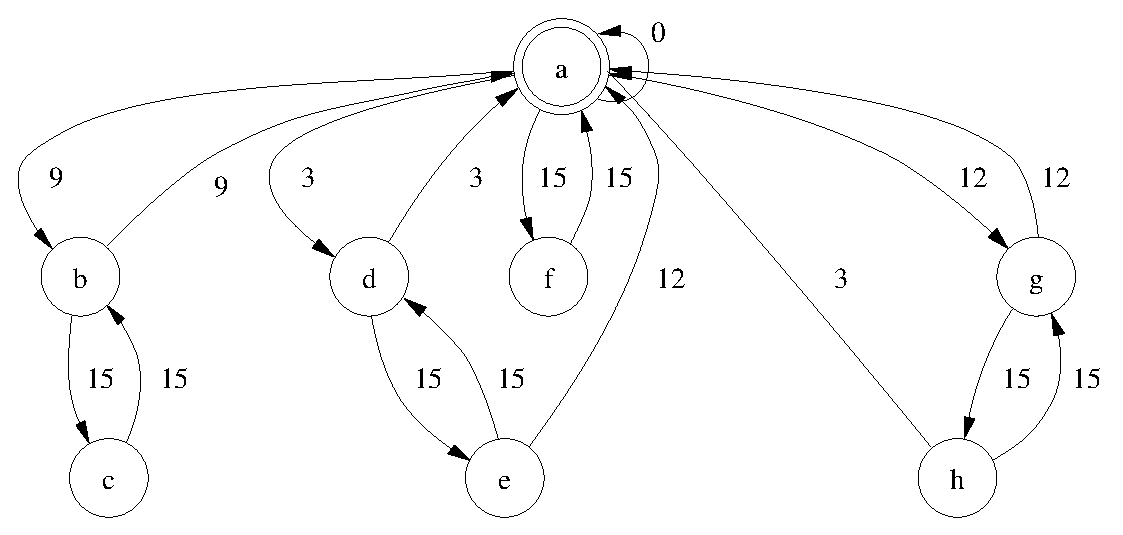
\includegraphics[scale=0.8]{abra.eps}
	\caption{\label{abra-automata} A $4\times m$-es tábla lefedéseinek mátrixreprezentációit felismerő automata}
\end{figure}


\chapter{Függelék}

\section{A program forráskódja}
A függelékbe kerülhetnek a hosszú táblázatok, vagy mondjuk egy programlista:
% A verbatim kornyezet hasznalatanal ügyeljünk rá, hogy az editor a szóközöjket át ne írja tab karakterekre!
\begin{verbatim}
   while (ujkmodosito[i]<0)
   {
      if (ujkmodosito[i]+kegyenletes[i]<0)
      {
         j=i+1;
         while (j<14)
         if (kegyenletes[i]+ujkmodosito[j]>-1) break;
         else j++;
         temp=ujkmodosito[j];
         for (l=i;l<j;l++) ujkmodosito[l+1]=ujkmodosito[l];
         ujkmodosito[i]=temp;
      }
      i++;
   }
\end{verbatim}


\chapter*{Nyilatkozat}
%Egy üres sort adunk a tartalomjegyzékhez:
\addtocontents{toc}{\ }
\addcontentsline{toc}{section}{Nyilatkozat}
%\hspace{\parindent}

% A nyilatkozat szövege más titkos és nem titkos dolgozatok esetében.
% Csak az egyik tipusú myilatokzatnak kell a dolgozatban szerepelni
% A ponok helyére az adatok értelemszerűen behelyettesídendők es
% a szakdolgozat /diplomamunka szo megfeleloen kivalasztando.


%A nyilatkozat szövege TITKOSNAK NEM MINŐSÍTETT dolgozatban a következő:
%A pontokkal jelölt szövegrészek értelemszerűen a szövegszerkesztőben és
%nem kézzel helyettesítendők:

\noindent
Alulírott \makebox[4cm]{\dotfill} szakos hallgató, kijelentem, hogy a dolgozatomat a Szegedi Tudományegyetem, Informatikai Intézet \makebox[4cm]{\dotfill} Tanszékén készítettem, \makebox[4cm]{\dotfill} diploma megszerzése érdekében.

Kijelentem, hogy a dolgozatot más szakon korábban nem védtem meg, saját munkám eredménye, és csak a hivatkozott forrásokat (szakirodalom, eszközök, stb.) használtam fel.

Tudomásul veszem, hogy szakdolgozatomat / diplomamunkámat a Szegedi Tudományegyetem Informatikai Intézet könyvtárában, a helyben olvasható könyvek között helyezik el.

\vspace*{2cm}

\begin{tabular}{lc}
	Szeged, \today\
	\hspace{2cm} & \makebox[6cm]{\dotfill} \\
	             & aláírás                 \\
\end{tabular}


\vspace*{4cm}

%A nyilatkozat szövege TITKOSNAK MINŐSÍTETT dolgozatban a következő:

\noindent
Alulírott \makebox[4cm]{\dotfill} szakos hallgató, kijelentem, hogy a dolgozatomat a Szegedi Tudományegyetem, Informatikai Intézet \makebox[4cm]{\dotfill} Tanszékén készítettem, \makebox[4cm]{\dotfill} diploma megszerzése érdekében.

Kijelentem, hogy a dolgozatot más szakon korábban nem védtem meg, saját munkám eredménye, és csak a hivatkozott forrásokat (szakirodalom, eszközök, stb.) használtam fel.

Tudomásul veszem, hogy szakdolgozatomat / diplomamunkámat a TVSZ 4. sz. mellékletében leírtak szerint kezelik.

\vspace*{2cm}

\begin{tabular}{lc}
	Szeged, \today\
	\hspace{2cm} & \makebox[6cm]{\dotfill} \\
	             & aláírás                 \\
\end{tabular}





\chapter*{Köszönetnyilvánítás}
\addcontentsline{toc}{section}{Köszönetnyilvánítás}

Ezúton szeretnék köszönetet mondani \textbf{X. Y-nak} ezért és ezért \ldots


%% Az itrodalomjegyzek keszitheto a BibTeX segedprogrammal:
%\bibliography{diploma}
%\bibliographystyle{plain}

%VAGY "kézzel" a következő módon:

\begin{thebibliography}{9}
	%10-nél kevesebb hivatkozás esetén

	%\begin{thebibliography}{99}
	% 10-nél több hivatkozás esetén

	\addcontentsline{toc}{section}{Irodalomjegyzék}

	%Elso szerzok vezetekneve alapjan ábécérendben rendezve.


	%folyóirat cikk: szerzok(k), a folyóirat neve kiemelve,
	%az evfolyam felkoveren, zarojelben az evszam, vegul az oldalszamok es pont.
	\bibitem{Gischer}
	J. L. Gischer,
	The equational theory of pomsets.
	\emph{Theoret. Comput. Sci.}, \textbf{61}(1988), 199--224.

	%könyv (szerzo(k), a könyv neve kiemelve, utana a kiado, a kiado szekhelye, az evszam es pont.)
	\bibitem{Pin}
	J.-E. Pin,
	\emph{Varieties of Formal Languages},
	Plenum Publishing Corp., New York, 1986.





\end{thebibliography}




\end{document}